\documentclass{beamer}
\usepackage{amsmath}
\usepackage{amsfonts}
\usepackage{amssymb}
\usepackage{verbatim}
\usepackage{graphicx}
\usepackage{subfig}
\usepackage{braket}
\usepackage{enumitem}
\setitemize{label=\usebeamerfont*{itemize item}%
  \usebeamercolor[fg]{itemize item}
  \usebeamertemplate{itemize item}}
\hfuzz=10pt
\vfuzz=50pt

\usepackage[justification=centering]{caption}
\captionsetup[figure]{labelformat=empty}% redefines the caption setup of the figures environment in the beamer class.

\usetheme{Rochester}
\setbeamertemplate{footline}[frame number]
%\setbeamertemplate{caption}{\raggedright\insertcaption\par}
%\usefonttheme[onlymath]{serif}
%\setbeamertemplate{caption}[numbered]
%\setbeamertemplate{enumerate items}[default]

\title{Boundary Effects in Stochastic Cyclic Competition Models on a Two-Dimensional Lattice}
\author{ M. Lazarus Arnau, Shannon Serrao, Uwe C. T\"auber }
\institute{ \vspace{-15pt}

    \small{Department of Physics, Center for Soft Matter and Biological Physics\\
    Virginia Tech}
}
\date{ \vspace{-15pt}

    \small{March 7, 2019} \\
    \vspace{-5pt}

        \begin{figure}[t]
            \centering
            %\raisebox{40pt}{
\includegraphics[height=55pt]{images/aro_logo_t.png}}
            \raisebox{0.5\height}{
\includegraphics[width=0.175\linewidth]{images/aro_logo_t.png}}
            \hfill
            %\raisebox{50pt}{
\includegraphics[height=35pt]{images/vt_logo.jpg}}
            \raisebox{1.5\height}{
\includegraphics[width=0.2\linewidth]{images/vt_logo.jpg}}
            \hfill
            %\raisebox{40pt}{
\includegraphics[height=55pt]{images/sps-logo.jpg}}
            \raisebox{0.5\height}{
\includegraphics[width=0.175\linewidth]{images/sps-logo.jpg}}
            %\label{fig:aro_logo_t}
        \end{figure}

    \vspace{-6pt}
}

\begin{document}
\beamertemplatenavigationsymbolsempty
    {
    \setbeamertemplate{footline}[default]
    \frame{\titlepage}
    }

    \begin{frame}[t]{Motivation}
        Three species cyclic competition schemes motivated by examples in biology, population dynamics, and chemistry.
        \vspace{-5pt}

        \begin{figure}[h]
            \centering
            %\subfloat[Rock Paper Scissors]{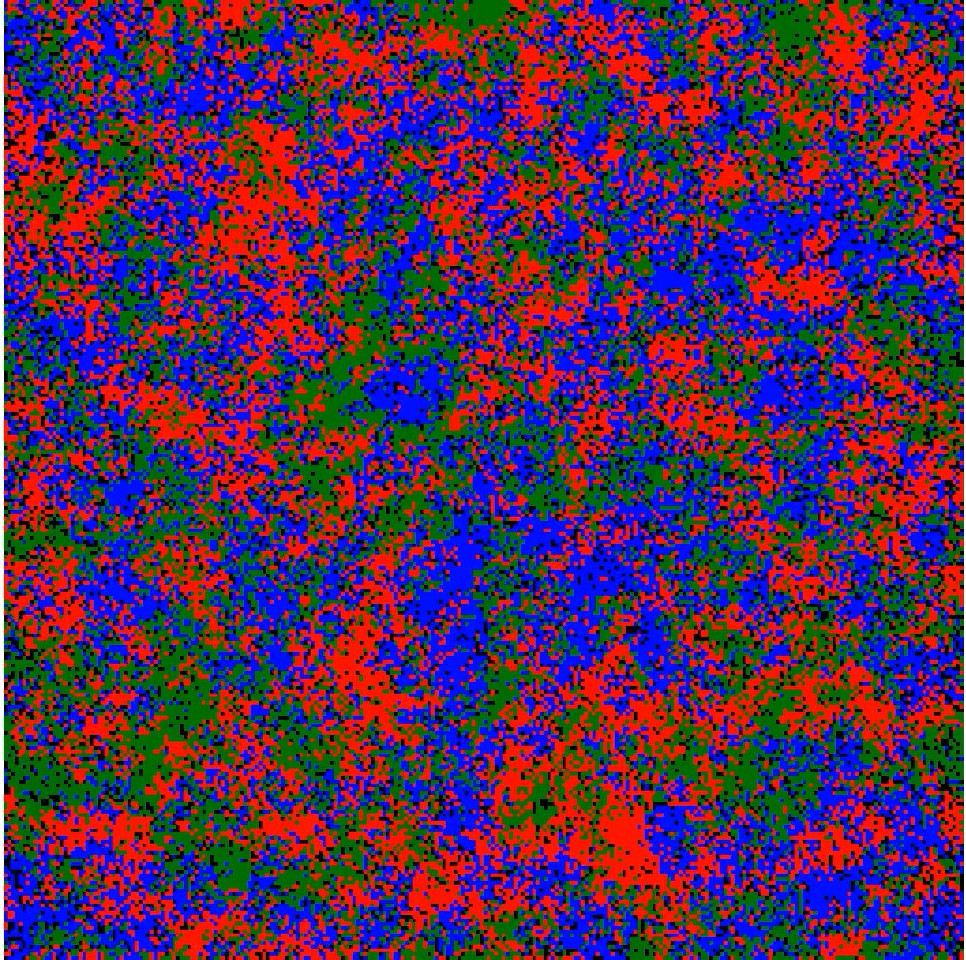
\includegraphics[height=0.7\textheight]{images/rps_1_25.jpg}}
            \subfloat[Rock Paper Scissors]{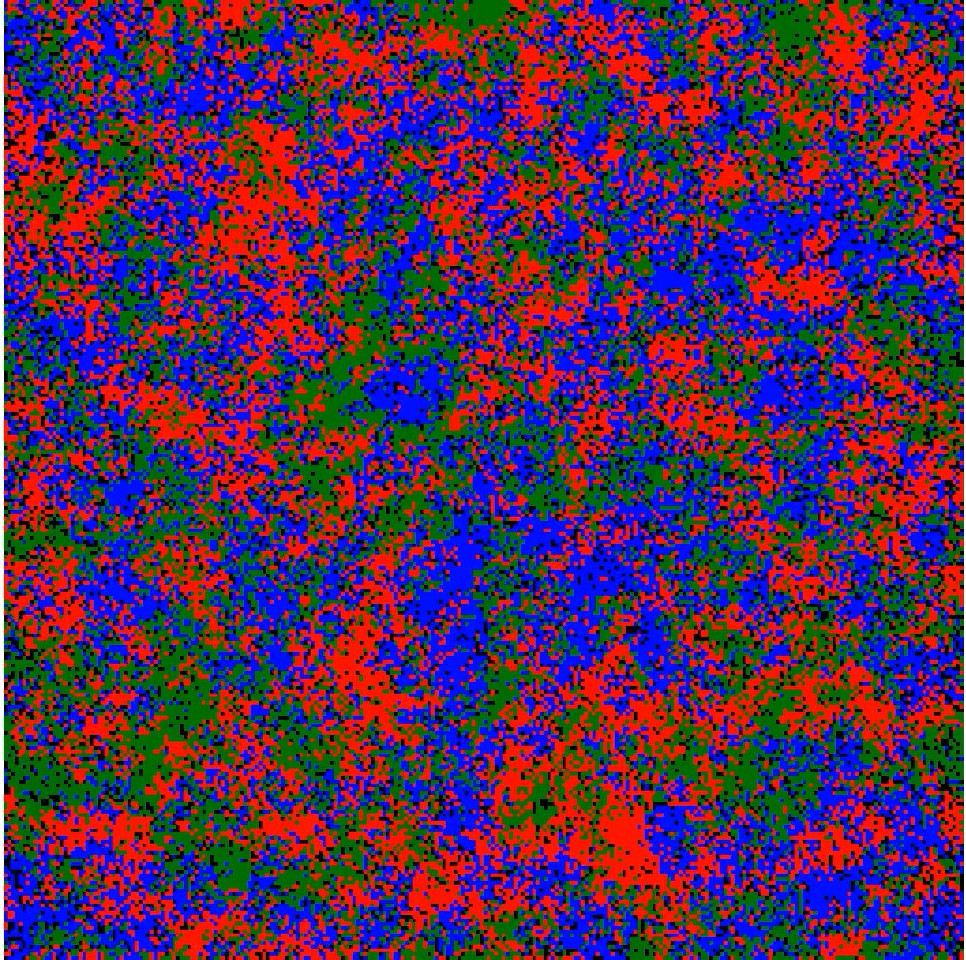
\includegraphics[width=0.5\linewidth]{images/rps_1_25.jpg}}
            %\subfloat[May-Leonard]{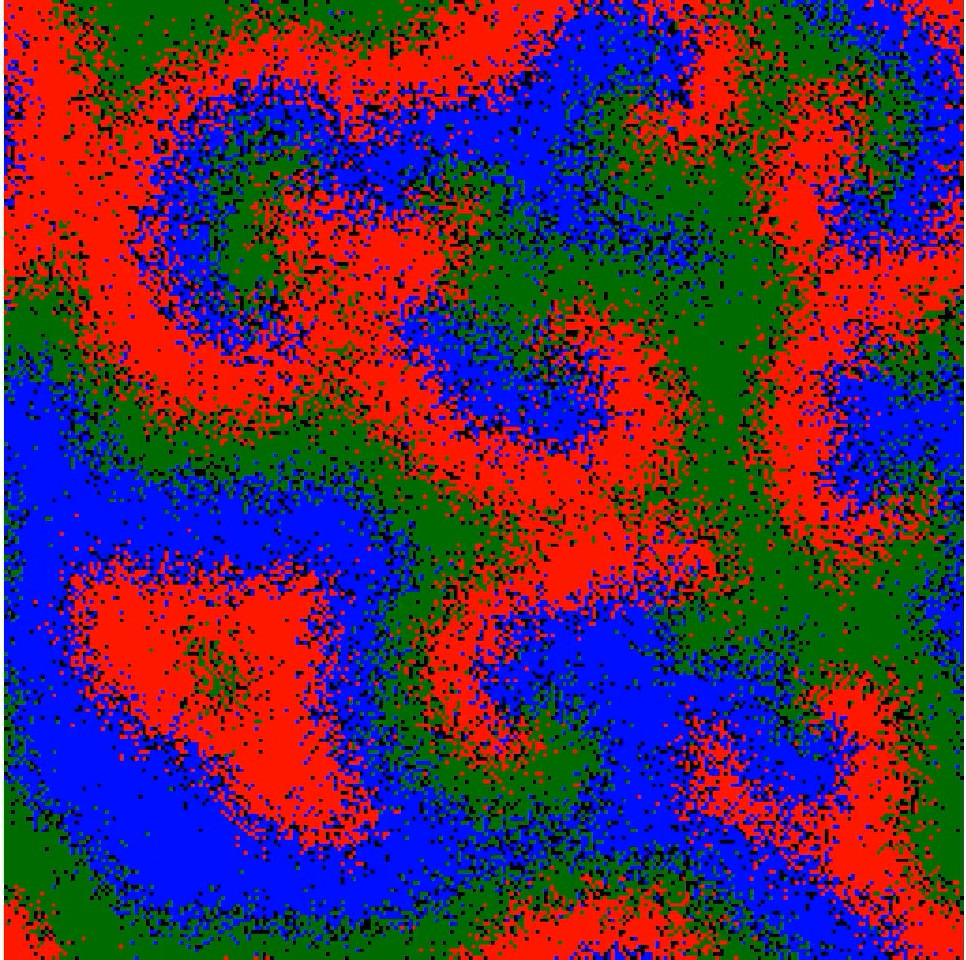
\includegraphics[height=0.7\textheight]{images/ml_5_0.jpg}}
            \subfloat[May-Leonard]{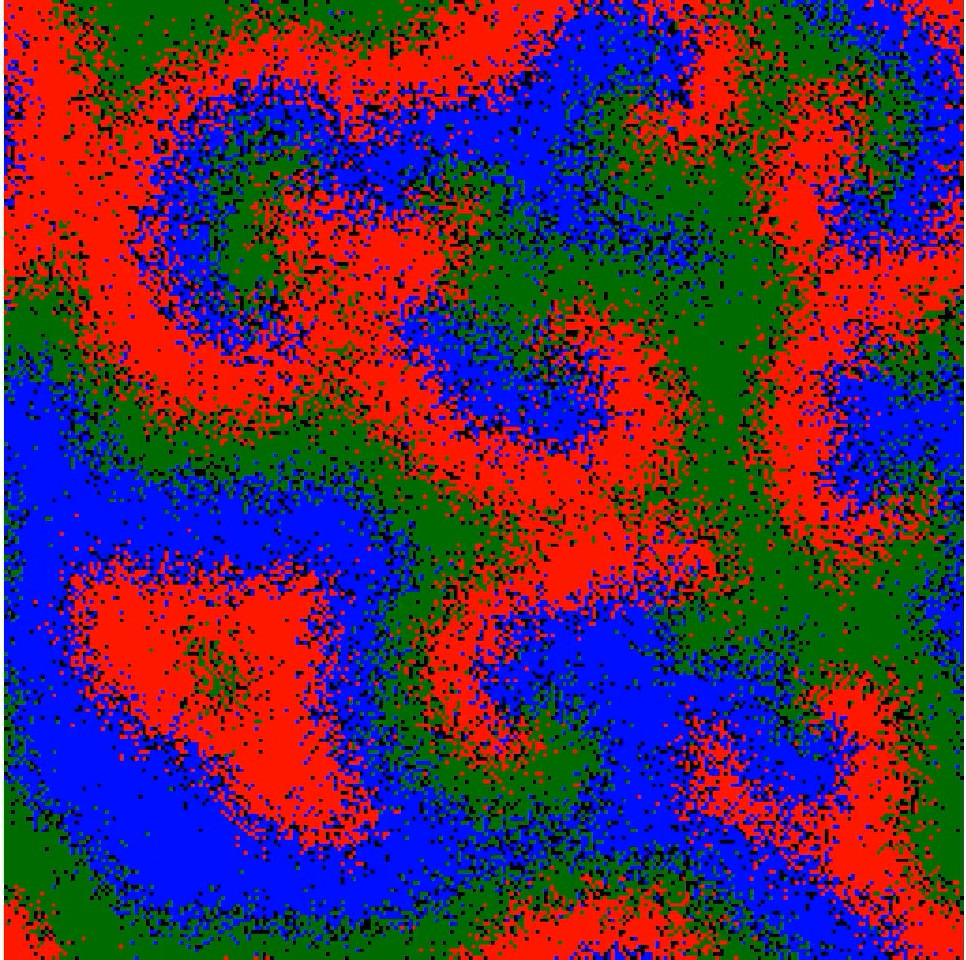
\includegraphics[width=0.5\linewidth]{images/ml_5_0.jpg}}
            %\caption{Typical steady state snapshots of Rock-Paper-Scissors (a) and May-Leonard (b) systems }
            \label{fig:name}
        \end{figure}
    \end{frame}
    \begin{frame}
        \frametitle{Models}

        %Three species cyclic competition schemes motivated by examples in biology, population dynamics, and chemistry.
                
        \begin{columns}
            \begin{column}{0.5\textwidth}
                \centering
                    Rock-Paper-Scissors/Cyclic Lotka-Volterra (RPS) Model
                        \begin{align*}
                            (\text{Replacement})  &
                            \left\{
                            \begin{matrix}
                            AB \xrightarrow{\alpha} AA\\
                            BC \xrightarrow{\alpha} BB\\
                            CA \xrightarrow{\alpha} CC\\
                            \end{matrix}
                            \right.\\
                            (\text{Pair-Swapping}) & \ XY \xrightarrow{\epsilon_r} YX \\
                        \end{align*}
            \end{column}
            \begin{column}{0.5\textwidth}
                \centering

                \vspace{-16pt}

                    May-Leonard (ML) Model
                        \begin{align*}
                            (\text{Predation}) & 
                            \left\{
                            \begin{matrix}
                            AB \xrightarrow{\alpha} A\varnothing\\
                            BC \xrightarrow{\alpha} B\varnothing\\
                            CA \xrightarrow{\alpha} C\varnothing\\
                            \end{matrix}
                            \right.\\
                            (\text{Reproduction}) & \ X \varnothing \xrightarrow{\alpha} XX \\
                            (\text{Pair-Swapping}) & \ XY \xrightarrow{\epsilon_m} YX 
                        \end{align*}
            \end{column}
        \end{columns}
        \begin{equation*}
            X \in \set{A, B, C}, \ Y \in \set{A, B, C, \varnothing}
        \end{equation*}
    \end{frame}

    \begin{frame}[t]{Combined System}
        \begin{columns}
            \begin{column}{0.5\textwidth}
                \begin{itemize}
                    \small{
                    \item Periodic boundary conditions (i.e. toroidal topology)
                    \item Maximum occupancy of one particle per lattice site.
                    \item May-Leonard except for thin (width $= 64 $) annular patch governed by RPS
                    \item Random initial conditions.
                    \item $ 512 \times 512 $ lattice sites.
                    \item $ \alpha = 1.0, \ \epsilon_m = 5.0 $. $ \epsilon_r $ varied between simulations
                    }
                \end{itemize}
            \end{column}
            \begin{column}{0.5\textwidth}
                \begin{figure}[h]
                    \centering
                    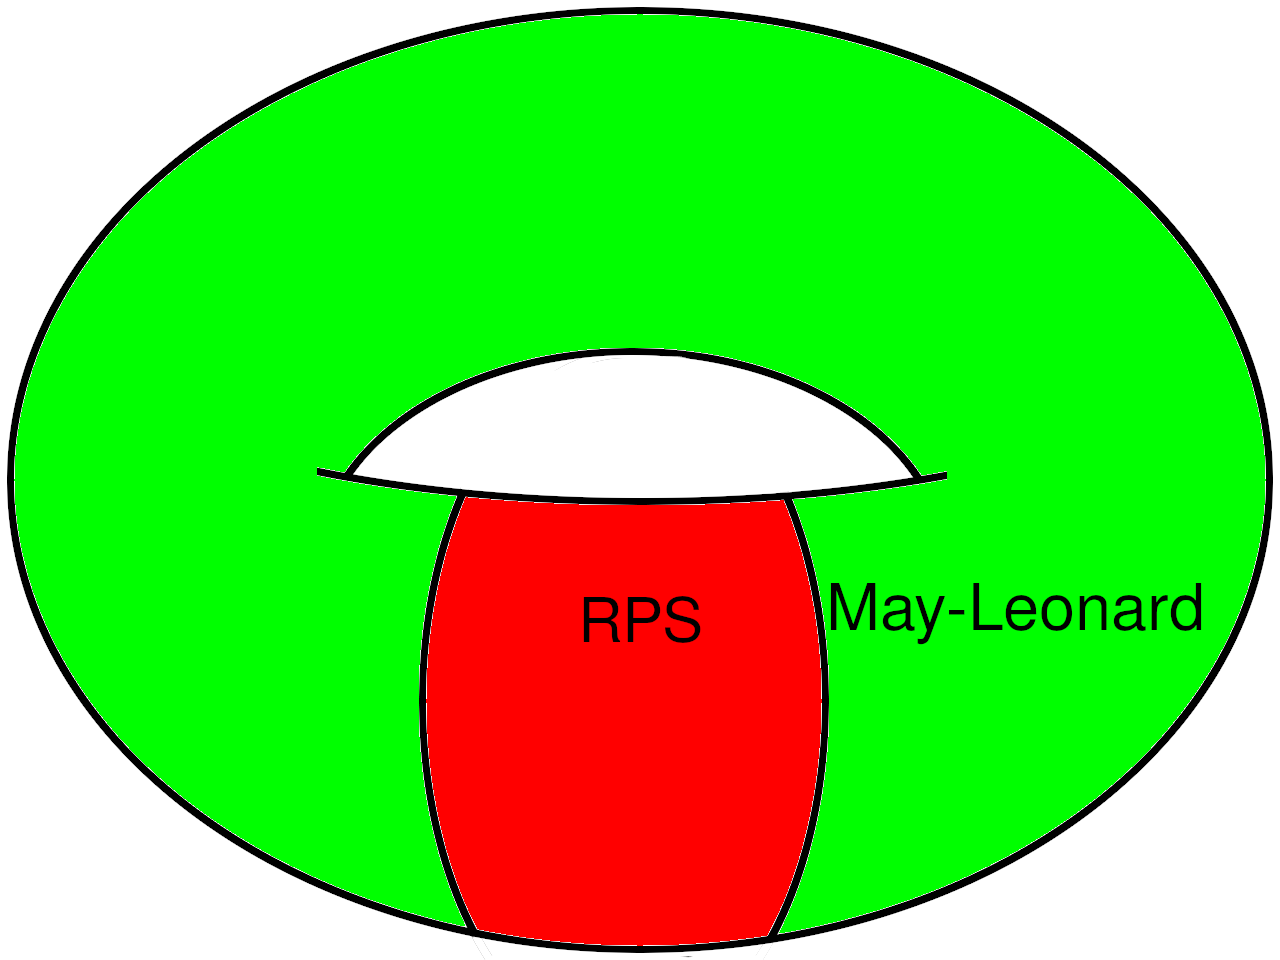
\includegraphics[width=\linewidth]{images/Model_Illustration.png}
                    \caption{System topolgy and layout}
                    \label{fig:plane_wave_2}
                \end{figure}
            \end{column}
        \end{columns}
    \end{frame}

    \begin{frame}
        \frametitle{Combined System}
        \begin{figure}[h]
            \centering
            \vspace{-5pt}

            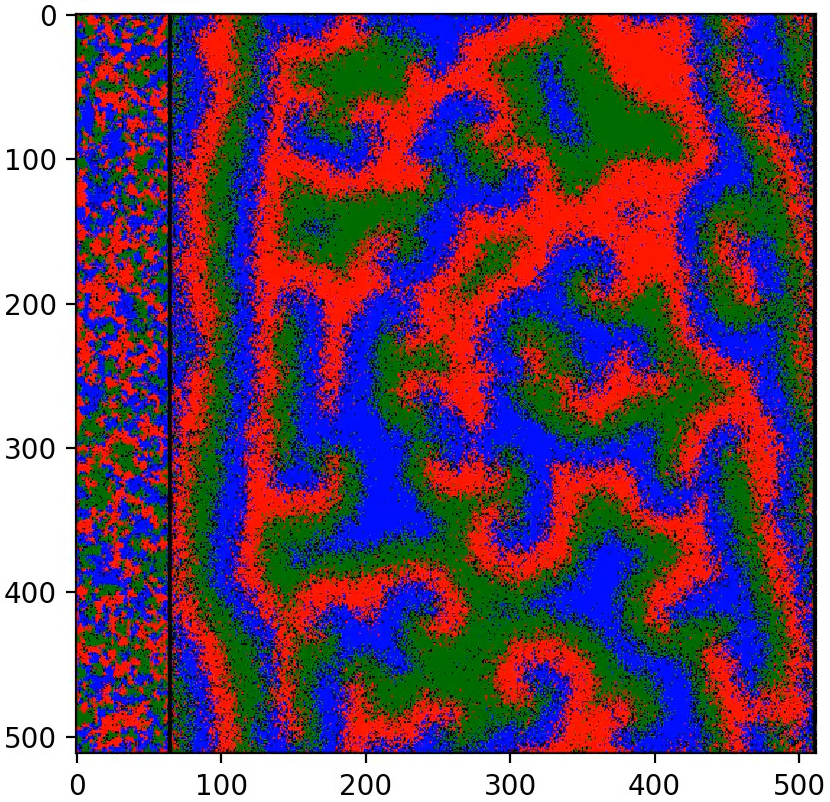
\includegraphics[height=\textheight]{images/plane_wave_new_2.jpg}
            %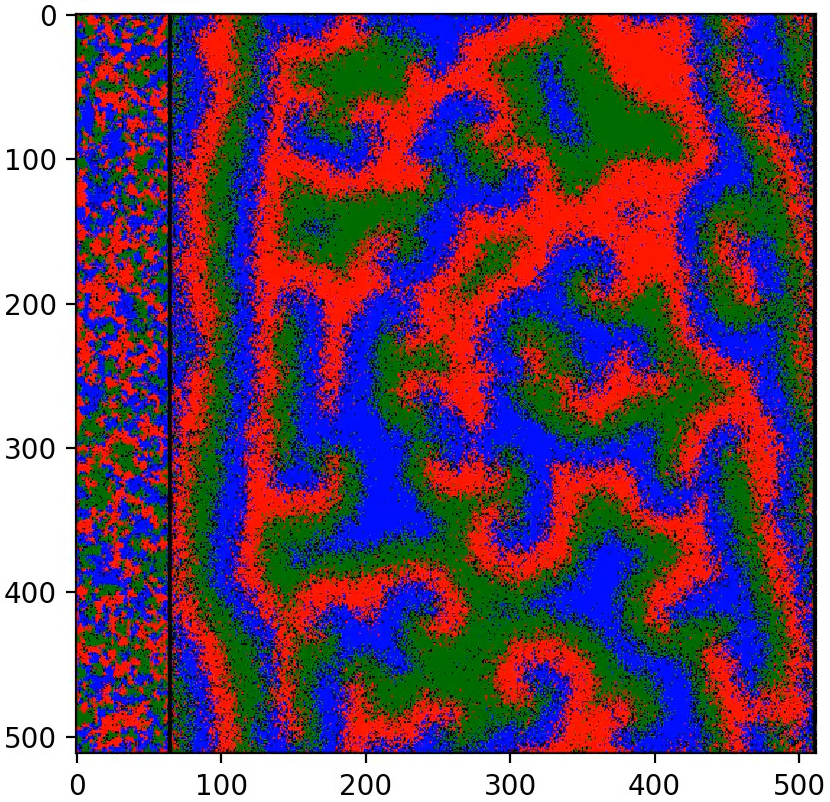
\includegraphics[width=\linewidth]{images/plane_wave_new_2.jpg}
            %\label{fig:plane_wave_2}
        \end{figure}
    \end{frame}

    \begin{frame}[t]{Correlation Lengths and Permeation Distance}
        \begin{columns}
            \begin{column}{0.3\textwidth}
                \vspace{-30pt}

                \begin{itemize}[leftmargin=1pt]
                \footnotesize
                    \item Vertical correlation function $ C(x,t, r) $ measured parallel
                        to interface.
                    \item $ C(x,t,r) $ averaged over multiple runs and used to calculate the vertical correlation length $ L(x) $.
                    \item Low $ \epsilon_r $ corresponds to higher $ L(x) $ near
                        interface.
                    \item Permeation distance of the plane-waves are approximately 
                        equal for all $ \epsilon_r $ tested
                \end{itemize}
            \end{column}
            \begin{column}{0.7\textwidth}
                
                \hfuzz=15pt
                \vspace{-15pt}

                %\hspace{10pt}
                \small{
                    %\begin{equation*}
                        %C(x,t,r) =  \frac{C_{AA}(x,t,r) + C_{BB}(x,t,r) + C_{CC}(x,t,r)}{3}  
                    %\end{equation*}
                \begin{align*}
                    \hfill
                    &C_{AA}(x,t,r) = \braket{n_a(x, y, t)n_a(x, y+r, t)} - (a(x, t))^2
                    \hspace{-20pt} \\
                    \hfill
                    &C(x,t,r) =  \frac{C_{AA}(x,t,r) + C_{BB}(x,t,r) + C_{CC}(x,t,r)}{3}  
                    \hspace{-20pt}
                \end{align*}
                }

                \vspace{-35pt}

                \begin{figure}[h]
                    \centering
                    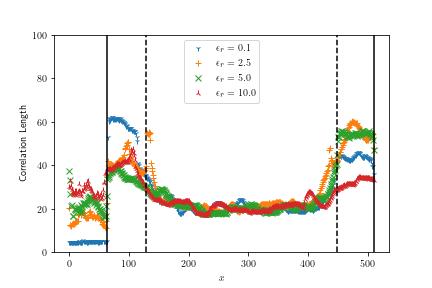
\includegraphics[height=0.72\textheight]{images/correlation_lengths.png}
                    %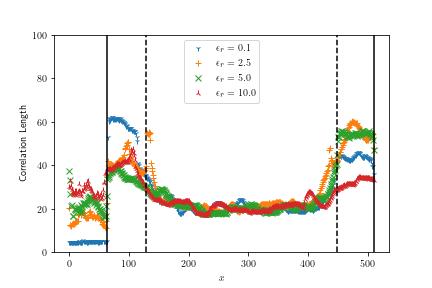
\includegraphics[width=\linewidth]{images/correlation_lengths.png}
                    %\caption{Correlation length}
                    \hspace{-30pt}
                    \label{fig:correlation_length}
                \end{figure}
            \end{column}
        \end{columns}
    \end{frame}

    %\begin{frame}[t]{Well-Mixing Effects}
        %\framesubtitle{Boundary Effects}
        %\vspace{-10pt}

        %\begin{figure}[h]
            %\centering
            %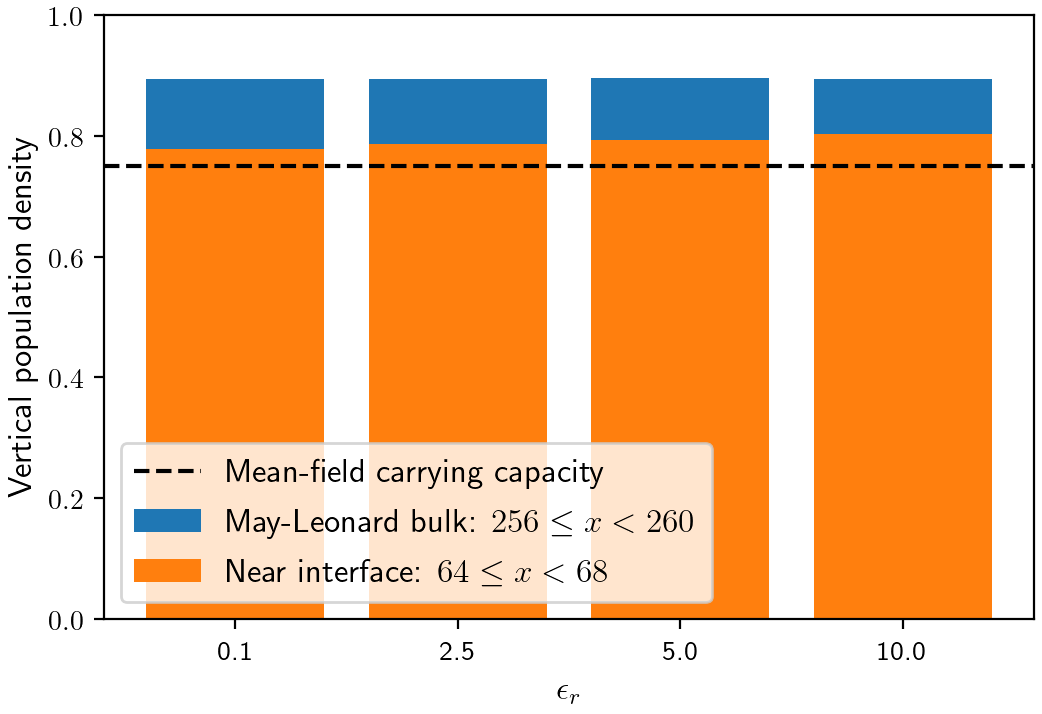
\includegraphics[width=0.95\linewidth]{images/density.png}

            %\vspace{-5pt}

            %\caption{Prominent drop in net population density near interface.}
            %\label{fig:mixing}
        %\end{figure}
    %\end{frame}

    %\begin{frame}[t]{Well-Mixing Effects}
        %\framesubtitle{Boundary Effects cont.}
        %\begin{figure}[h]
            %\centering
            %\vspace{-15pt}

            %{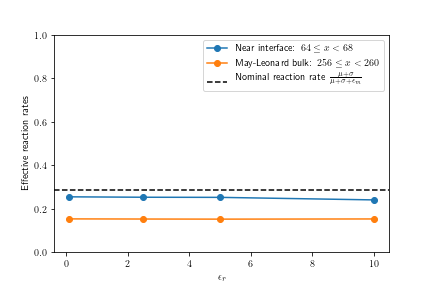
\includegraphics[width=\linewidth]{images/reaction_rates.png}}
            %\vspace{-20pt}

            %\caption{ Relative reproduction $+$ predation rates near the boundary 
            %vs. in ML bulk}
            %\label{fig:mixing}
        %\end{figure}
    %\end{frame}

    \begin{frame}[t]{Well Mixing Effects}
        \begin{columns}
            \begin{column}{0.5\textwidth}
                
                \vspace{20pt}

                \begin{figure}[h]
                    \centering
                    %\hspace{15}
                    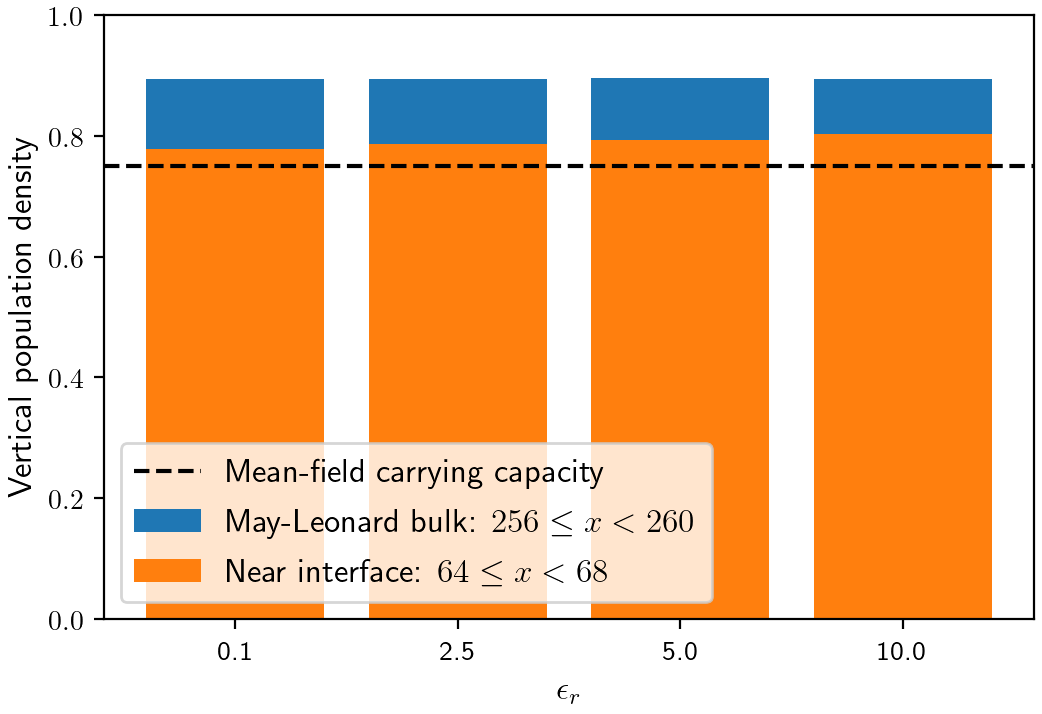
\includegraphics[width=\linewidth]{images/density.png}

                    %\vspace{0pt}

                    \caption{Average net population densities near and far from the RPS-ML interface
                    for various RPS mobility rates.}
                    %\label{fig:mixing}
                \end{figure}
            \end{column}
            \begin{column}{0.5\textwidth}
                
                \vspace{5pt}

                \begin{figure}[h]
                    \centering
                    %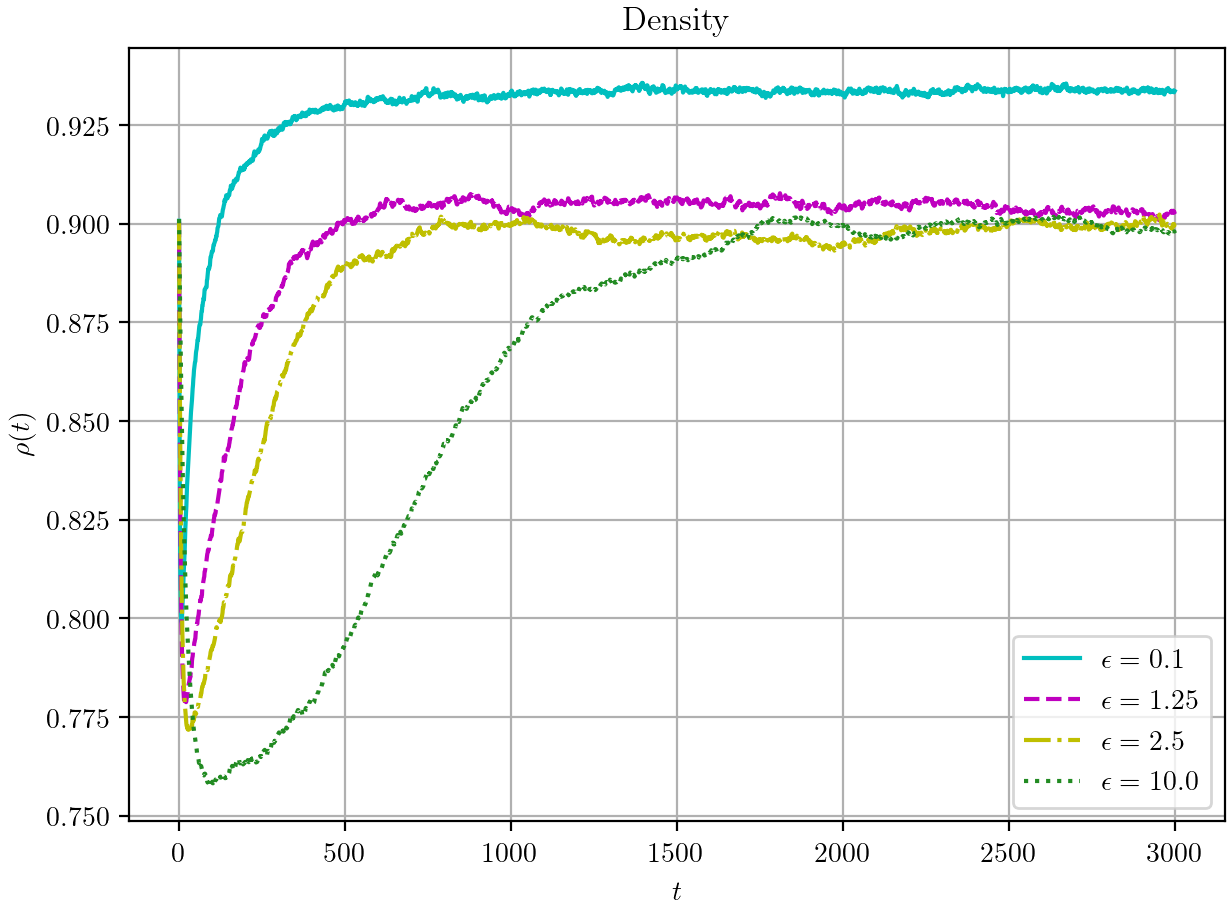
\includegraphics[height=0.9\textheight]{images/densities_try_0.png}
                    %\hspace{-25pt}
                    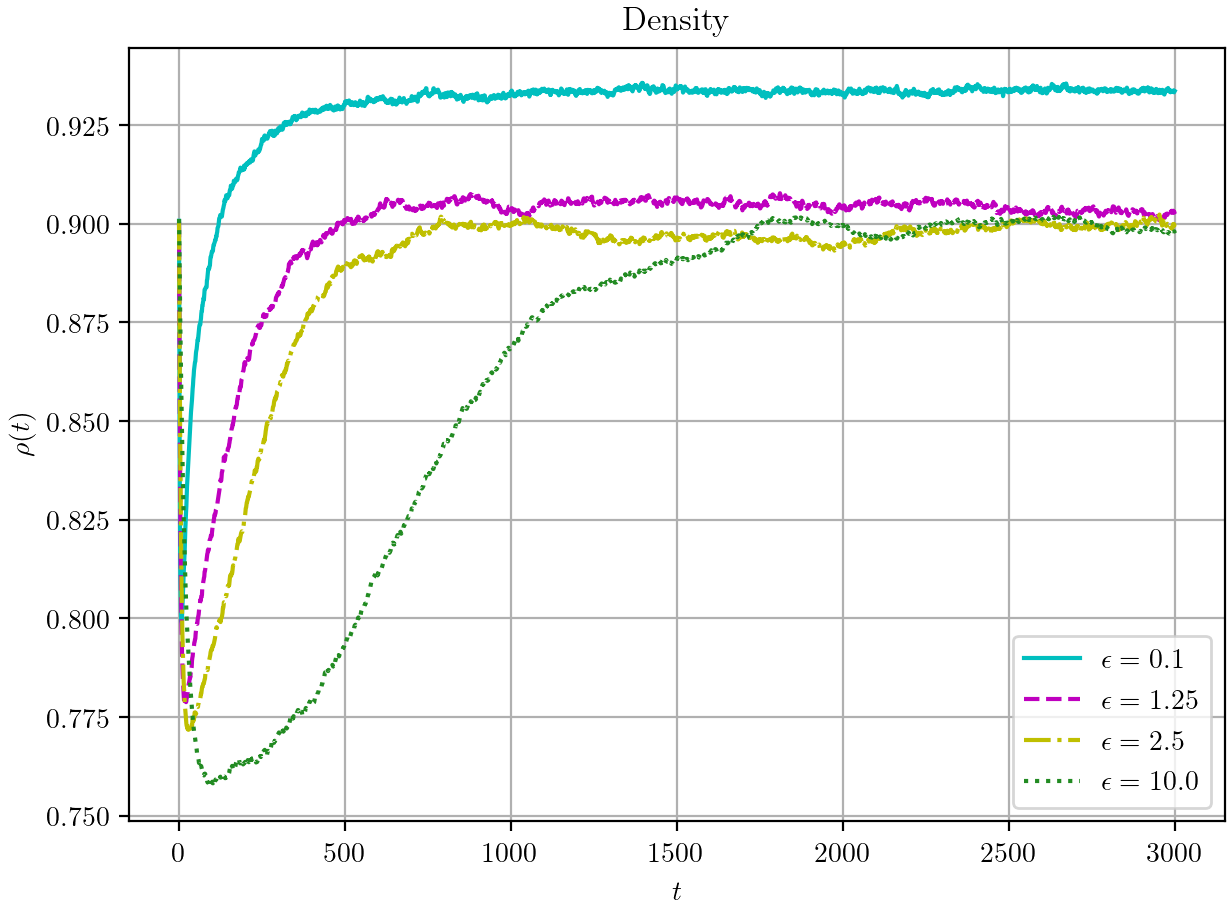
\includegraphics[width=1\linewidth]{images/densities_try_0.png}

                    \vspace{0pt}

                    \caption{Net population density vs. time of pure ML lattice starting from from random initial
                    condition}
                    %\label{fig:images/densities_try_0}
                \end{figure}
            \end{column}
        \end{columns}
        
    \end{frame}

    %\begin{frame}[t]{Well-Mixing Effects}
        %\framesubtitle{Transient Effects}

        %\vspace{-15pt}

        %\begin{figure}[h]
            %\centering
            %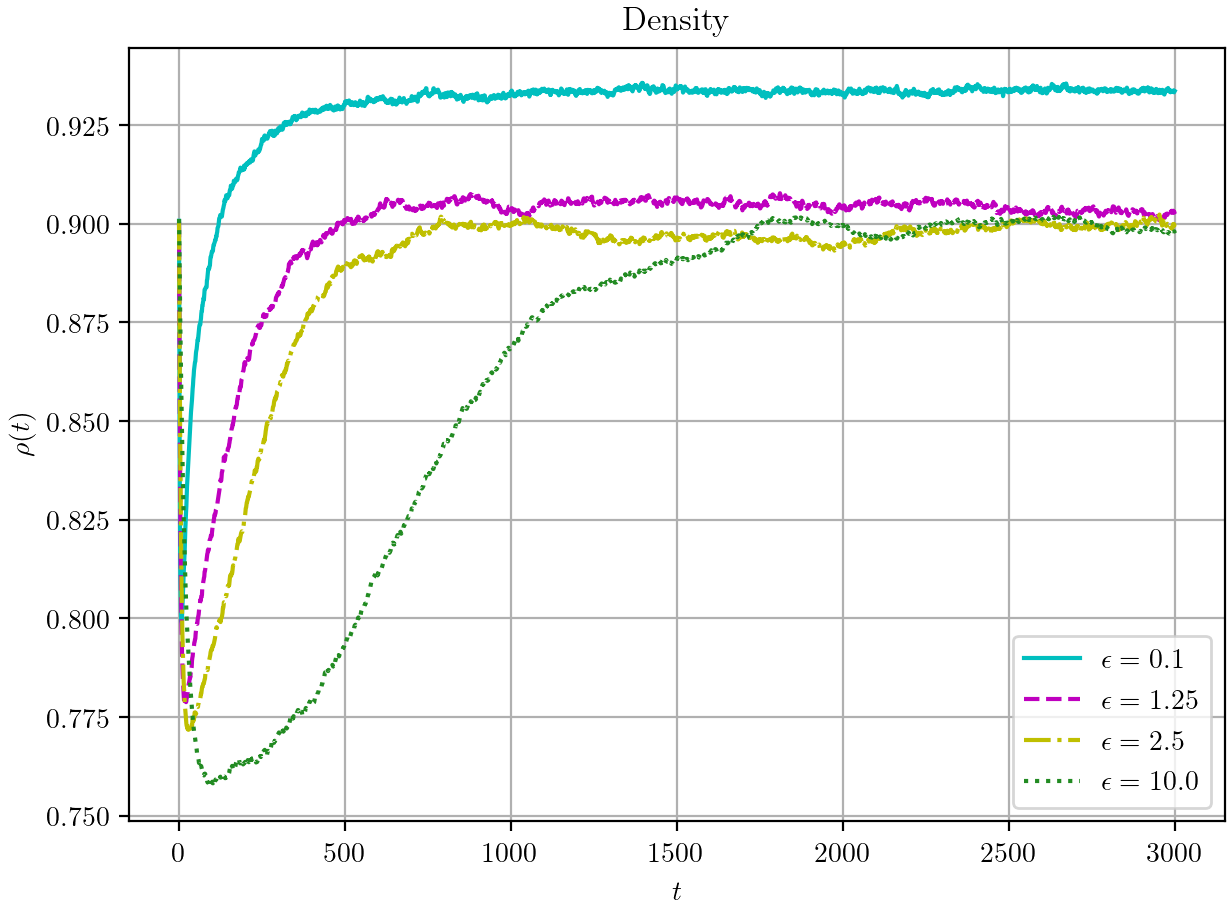
\includegraphics[height=0.9\textheight]{images/densities_try_0.png}
            %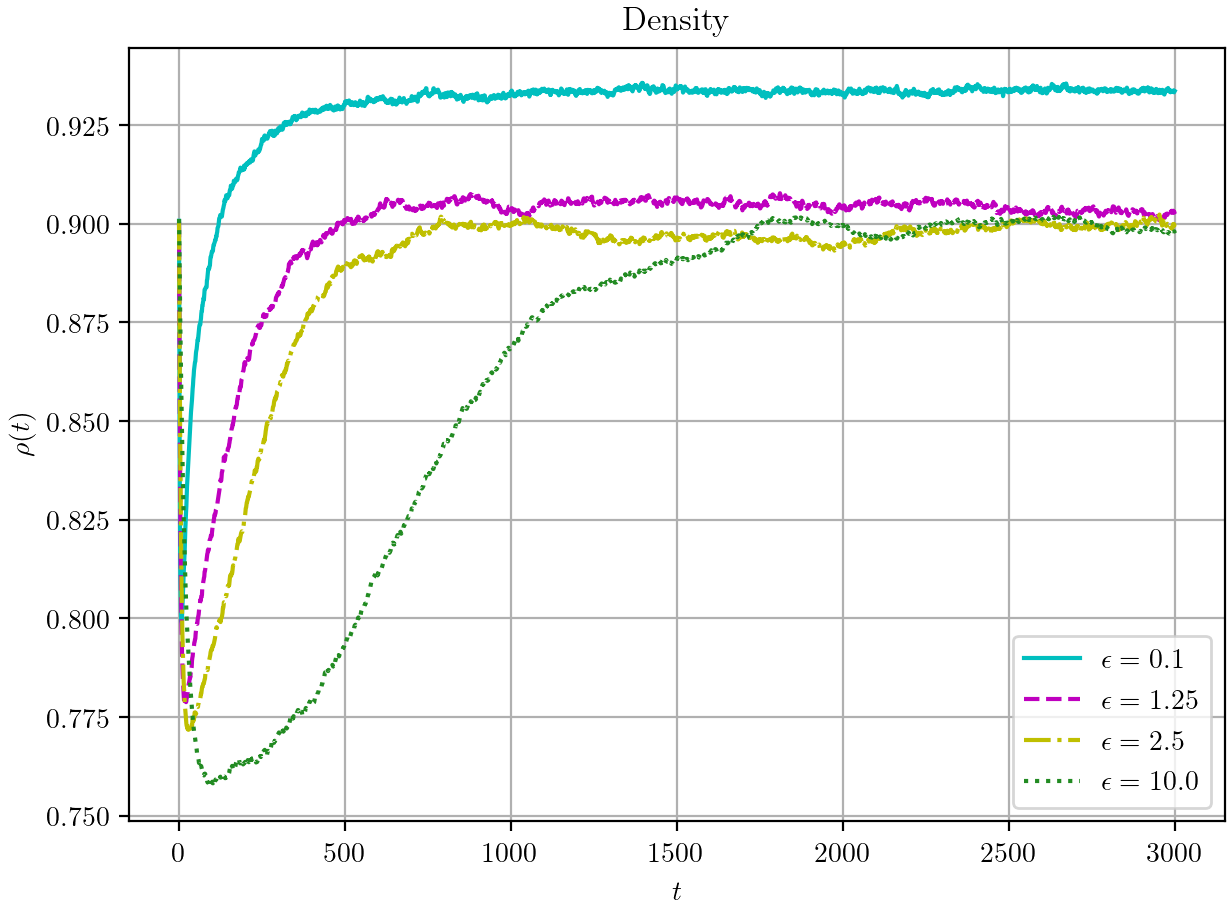
\includegraphics[width=0.7\linewidth]{images/densities_try_0.png}

            %\vspace{-5pt}

            %\caption{ From random initial conditions a pure ML model approaches mean-field 
                %population density before reaching its steady state carrying capacity.}
            %\label{fig:images/densities_try_0}
        %\end{figure}
    %\end{frame}

    \begin{frame}[t]{Conclusions}
                
        \begin{itemize}
            \item Changing the microscopic rules from ML to RPS on a subsection of the lattice
                produces plane-waves emanating away from the interface.
            \item Size of the plane waves is apparently dependant on RPS mobility
            \item Drop in net population density near the interface due to the system
                being more ``well-mixed''.
            \item Suggests periodic, localized mixing as a potential method for disruption 
                of steady-state pattern formation in cyclic competition models.
        \end{itemize}

            \vspace{10pt}

            \footnotesize {Research was sponsored by the Army Research Office and was
                accomplished under Grant Number W911NF-17-1-0156.

                \vspace{5pt}

                Additional travel support from Society of Physics Students Travel Award
            }

    \end{frame}
\end{document}


